\scanpage{73}
$S$ \inserted{lisse} de \deleted{\unsure{f}} type fini sur $\mathbb{F}_p$ % 1

$M$ motif ct tordu de poids $\rho$ % 2
\[
 ?\;-\; H^*(S,M_\ell)\overset{?}{\Leftarrow}
 H^p(\mathbb{F}_p,R^q f_*(M_\ell)) % 3
\]
\[
\begin{aligned}
0\to{}&
\underbrace{H^{\unsure{i-1|i}}(\bar S,\bar M_\ell)_{\pi}}_{
 \substack{\text{poids entre}\\\rho+i-1\ \text{et }\rho+\operatorname{Inf}(\unsure{2i-2|2i-1},2n)}}
\longrightarrow H^{\deleted{\unsure{n}}i}(S,M_\ell)\longrightarrow
\underbrace{H^{\deleted{\unsure{n}}i}(\bar S,\bar M_\ell)^{\pi}}_{
 \substack{\text{poids entre}\\\rho+i\ \text{et }\rho+\operatorname{Inf}(2i,2n)}}\;-\;0 % 4–6
\end{aligned}
\]
Donc $H^i(S,M_\ell)=0$ \deleted{si on a} sauf si on a % 7
\[
\begin{aligned}
&\rho+i-1\le 0\le\rho+2i-2 &&\text{\uline{ou}}\quad \rho+i\le0\le\rho+2i\\ % 8
\deleted{\unsure{\rho}}\ \text{i.e.}\quad&2-2i\le\rho\le\deleted{\unsure{2i}}1-i
 &&\text{\uline{ou}}\quad -2i\le\rho\le-i\\ % 9
\text{i.e.}\quad&-2i\le\rho\le-i+1 &&(\deleted{\unsure{\rho}}\ \text{si }i\ge2)\\ % 10
&-2\le\rho\le1 &&(\text{si }i=1)\\ % 11
&\rho=0 &&(\text{si }i=0) % 12
\end{aligned}
\]
\deleted{Pour $i=1$, cela \unsure{donne}} % 13

$\unsure{\rho|?}$ % 14

\figure{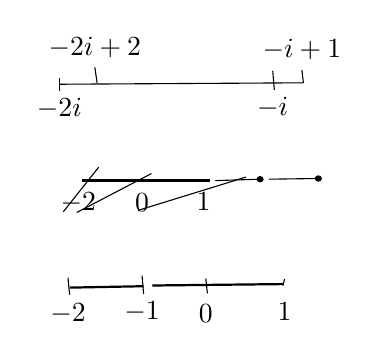
\begin{tikzpicture}[x=1cm,y=.9cm]
\draw (0,0)--(3.1,.02);
\draw (0,-.09)--(0,.09) node[below=4pt] {$-2i$};
\draw (.48,.02)--(.45,.24) node[above] {$-2i+2$};
\draw (2.73,-.08)--(2.71,.19) node[below=6pt] {$-i$};
\draw (3.1,.02)--(3.08,.2) node[above] {$-i+1$};
\draw[very thick] (.29,-1.36)--(1.91,-1.36);
\draw (1.98,-1.36)--(2.55,-1.34) (2.66,-1.34)--(3.29,-1.33);
\fill (2.55,-1.34) circle (.045) (3.29,-1.33) circle (.045);
\node at (.24,-1.67) {$\deleted{\unsure{-2}}$};
\node at (1.05,-1.67) {$\deleted{\unsure{0}}$};
\node at (1.83,-1.66) {$\deleted{\unsure{1}}$};
\draw (.05,-1.8)--(.5,-1.17) (.22,-1.81)--(1.17,-1.26)
 (1.00,-1.78)--(2.37,-1.31);
\draw[thick] (.13,-2.87)--(1.07,-2.85) (1.18,-2.84)--(2.85,-2.82);
\draw (.13,-2.97)--(.11,-2.73) node[below=6pt] {$-2$};
\draw (1.07,-2.96)--(1.05,-2.70) node[below=6pt] {$-1$};
\draw (1.88,-2.95)--(1.86,-2.74) node[below=6pt] {$0$};
\draw (2.84,-2.84)--(2.86,-2.75) node[below=5pt] {$1$};
\end{tikzpicture}} % 15–17
% archive sheet number: 72
